\pagebreak
\thispagestyle{empty}
\movetoevenpage
\begin{figure}
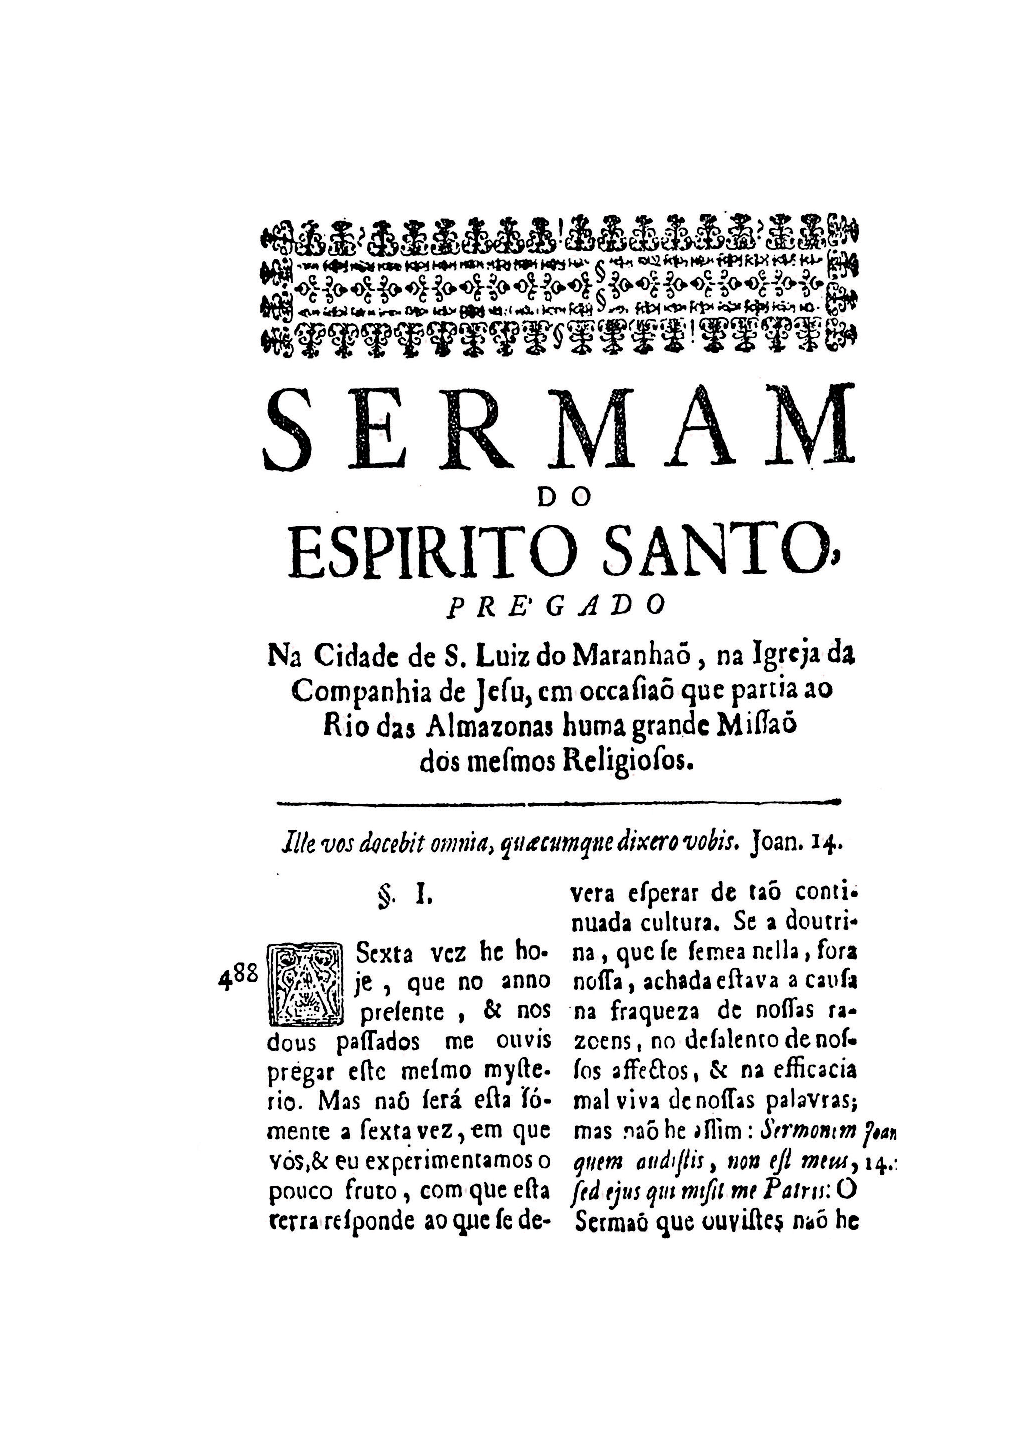
\includegraphics[width=\textwidth]{./imgs/espirito.pdf}  
\end{figure}

\chapter{Sermão do Espírito Santo}

\begin{quotation}
\noindent{}Pregado na Cidade de São Luís do Maranhão, na Igreja da Companhia de Jesus,
em ocasião que partia ao Rio das Amazonas uma grande Missão dos mesmos Religosos.
\end{quotation}

\epigraph{\emph{Ille vos docebil omnia, quaecumque dixero vobis}.}{Jo, 14.}


\section{i}

\noindent{}A sexta vez é hoje, que no ano presente e nos dois passados me ouvis
pregar este mesmo mistério. Mas não será esta somente a sexta vez em que
vós e eu experimentamos o pouco fruto com que esta terra responde ao que
se devera esperar de tão continuada cultura. Se a doutrina que se semeia
nela fora nossa, achada estava a causa na fraqueza de nossas razões, no
desalento de nossos afetos e na eficácia mal viva de nossas palavras;
mas não é assim: \emph{Sermonem quem audistis non est meus, sed ejus qui
misit me, Patris}: O sermão que ouvistes não é meu, senão % (Jo. 14, 24)
do Eterno Padre que me mandou ao mundo (diz Cristo neste Evangelho)
e o mesmo podem dizer todos os pregadores, ao menos os que ouvis
deste lugar. Os sermões, as verdades, a doutrina que pregamos não é
nossa, é de Cristo. Eles a disse, os evangelistas a escreveram, nós a
repetimos. Pois, se estas repetições são tantas e tão continuadas, e a
doutrina que pregamos não é nossa, senão de Cristo, como fazem tão
poucos progressos nela, e como aprendem tão pouco os que a ouvem? Nas
palavras que propus temos a verdadeira resposta desta tão nova
admiração.

\emph{Ille vos docebit omnia quaecumque dixero vobis}: O Espírito Santo,
diz Cristo, vos ensinará tudo o que eu vos tenho dito. Notai
a diferença dos termos, e vereis quanto vai de dizer a ensinar. Não diz
Cristo: o Espírito Santo vos dirá o que eu vos tenho dito; nem diz: o
Espírito Santo vos ensinará o que eu vos tenho ensinado; mas diz: O
Espírito Santo vos ensinará o que eu vos tenho dito, porque o pregador,
ainda que seja Cristo, diz: o que ensina é o Espírito Santo. Cristo diz:
\emph{Quaecumque dixero vobis}; o Espírito Santo ensina: \emph{Ille vos
docebit omnia}. O mestre na cadeira diz para todos, mas não ensina a
todos. Diz para todos, porque todos ouvem; mas não ensina a todos,
porque uns aprendem, outros não. E qual é a razão desta diversidade, se
o mestre é o mesmo e a doutrina a mesma? Porque, para aprender, não
basta só ouvir por fora: é necessário entender por dentro. Se a luz de
dentro é muita, aprende"-se muito; se pouca, pouco; se nenhuma, nada. O
mesmo nos acontece a nós. Dizemos, mas não ensinamos, porque dizemos por
fora; só o Espírito Santo ensina, porque alumia por dentro:
\emph{Ministeria forinsecus adjutoria sunt, cathedram in caelo habet,
quia corda docet}, diz Santo Agostinho. Por isso até o mesmo Cristo,
pregando tanto, converteu tão pouco. Se o Espírito Santo não alumia por
dentro, todo o dizer, por mais divino que seja, é dizer:
\emph{Quaecumque dixero vobis}; mas se as vozes exteriores são
assistidas dos raios interiores da sua luz, logo qualquer que seja o
dizer, e de quem quer que seja, é ensinar, porque só o Espírito Santo é
o que ensina: \emph{Ille vos docebit}.

Por que vos parece que apareceu o Espírito Santo hoje sobre os
apóstolos, não só em línguas, mas em línguas de fogo? Porque as línguas
falam, o fogo alumia. Para converter almas, não bastam só palavras: são
necessárias palavras e luz. Se quando o pregador fala por fora, o
Espírito Santo alumia por dentro, se quando as nossas vozes vão aos
ouvidos, os raios da sua luz entram ao coração, logo se converte o
mundo. Assim sucedeu em Jerusalém neste mesmo dia. Sai S.\,Pedro do
cenáculo de Jerusalém, assistido deste fogo divino, toma um passo do
profeta Joel, declara"-o ao povo, e, sendo o povo a que pregava aquele
mesmo povo obstinado e cego, que poucos dias antes tinha crucificado a
Cristo, foram três mil os que naquela pregação o confessaram por
verdadeiro Filho de Deus e se converteram à fé. Oh! admirável eficácia
da luz do Espírito Santo! Oh! notável confusão vossa e minha! Um
pescador, com uma só pregação e com um só passo da Escritura, no dia de
hoje converte três mil infiéis, e eu, no mesmo dia, com cinco e com seis
pregações, com tantas Escrituras, com tantos argumentos, com tantas
razões, com tantas evidências, não posso persuadir um cristão. Mas a
causa é porque eu falo e o Espírito Santo, por falta de disposição
nossa, não alumia. Divino Espírito, não seja a minha indignidade a que
impeça a estas almas, por amor das quais descestes do céu à terra, o
fruto de vossa santíssima vinda: \emph{Veni Sancte Spiritus, et emitte
caelitus lucis tuae radium}: Vinde, Senhor, e mandai"-nos do céu um raio
eficaz de vossa luz: não pelos nossos merecimentos, que conhecemos
quão indignos são, mas pela infinita bondade vossa, e pela intercessão
de vossa esposa santíssima. Ave Maria.

\section{ii}

\emph{Ille vos docebit omnia}. Diz Cristo aos apóstolos que o Espírito
Santo os ensinará. E ser Cristo, ser o Filho de Deus o que diz estas
palavras, faz segunda dificuldade à inteligência e razão delas. Ao Filho
de Deus, que é a segunda Pessoa da Santíssima Trindade, atribui"-se a
sabedoria; ao Espírito Santo, que é a terceira Pessoa, o amor; e suposto
isto parece que a Pessoa do Espírito Santo havia de encomendar o ofício
de ensinar à Pessoa do Filho, e não o Filho ao Espírito Santo. Que o
amor encomende o ensinar à sabedoria, bem está; mas a sabedoria
encomendar o ensinar ao amor: \emph{Ille vos docebit}? Neste caso sim.
Porque para ensinar homens infiéis e bárbaros, ainda que é muito
necessária a sabedoria, é muito mais necessário o amor. Para ensinar,
sempre é necessário amar e saber, porque quem não ama não quer, e quem
não sabe não pode; mas esta necessidade de sabedoria e amor não é sempre
com a mesma igualdade. Para ensinar nações fiéis e políticas, é
necessário maior sabedoria que amor;
para ensinar nações bárbaras e incultas, é necessário maior amor que
sabedoria. A segunda Pessoa, o Filho, e a terceira, o Espírito Santo,
ambas vieram ao mundo a ensinar e salvar almas; mas a missão do Filho
foi a uma nação fiel e política, e a missão do Espírito Santo foi
principalmente a todas as nações incultas e bárbaras. A missão do Filho
foi só a uma nação fiel e política, porque foi só aos filhos de Israel,
como o mesmo Senhor disse: \emph{Non sum missus nisi ad oves quae
perierunt domus Israel}. A missão do Espírito Santo foi principalmente
às nações incultas e bárbaras, porque foi para todas as nações do mundo,
que por isso desceu e apareceu em tanta diversidade de línguas:
\emph{Apparuerunt dispertitae linguae}. E como a primeira missão era
para uma nação política, e a segunda para todas as nações bárbaras, por
isso foi muito conveniente que à primeira viesse uma Pessoa divina, a
quem se atribui, não o amor, senão a sabedoria, e que à segunda viesse
outra pessoa, também divina, a quem se atribui, não a sabedoria, senão o
amor. Para ensinar homens entendidos e políticos, pouco amor é
necessário: basta muita sabedoria; mas para ensinar homens bárbaros e
incultos, ainda que baste pouca sabedoria, é necessário muito amor.

Desceu hoje o Espírito Santo em línguas, para formar aos apóstolos
mestres e pregadores, mas mestres e pregadores de quem? O mesmo Cristo
que os mandou pregar o disse: \emph{Euntes in mundum universum,
praedicate Evangelium omni creaturae}: Ide por todo o % (Mc. 16, 15)
mundo, e pregai a toda a criatura.
A toda a criatura, Senhor? É reparo de S.\,Gregório papa. Bem
sei eu que são criaturas os homens, mas os brutos animais, as árvores e
as pedras também são criaturas. Pois, se os apóstolos hão de pregar a
todas as criaturas, hão de pregar também aos brutos? Hão de pregar
também aos troncos? Hão de pregar também às pedras? Também, diz Cristo:
\emph{Omni creaturae}; não porque houvessem os apóstolos de pregar às
pedras, e aos troncos, e aos brutos, mas porque haviam de pregar a todas
as nações e línguas bárbaras e incultas do mundo, entre as quais haviam
de achar homens tão irracionais como os brutos, e tão insensíveis como
os troncos, e tão duros e estúpidos como as pedras. E para um apóstolo
se pôr a ensinar e abrandar uma pedra, para se pôr a ensinar e moldar um
tronco, para se pôr a ensinar e meter em juízo um bruto, vede se é
necessário muito amor de Deus. Em um deles o veremos.

Poucos dias antes de Cristo mandar aos apóstolos a pregar pelo mundo,
fez esta pergunta a S.\,Pedro: \emph{Simon Joannis, diligis me plus his}?%(Jo.21,15)
 Pedro, amas"- me mais que todos estes? Respondeu o santo:
\emph{Etiam, Domine, tu scis quia amo te}: Senhor, bem sabeis vós que
vos amo. Ouvida a resposta, torna Cristo a fazer segunda vez a mesma
pergunta: Simon \emph{Joannis, diligis me plus his}? Pedro, amas"- me
mais que todos estes? Respondeu S.\,Pedro, com a mesma submissão e
encolhimento, que bem sabia o Senhor, que o amava: \emph{Tu scis quia
amo te}. Ouvida a mesma resposta segunda vez, torna Cristo terceira vez
a repetir a mesma pergunta, e diz o texto que se entristeceu São Pedro:
\emph{Contristatus est Petrus, quia dixit ei tertio, amas me}? Entristeceu"-se Pedro,
porque Cristo lhe perguntou a terceira vez se o amava. E
verdadeiramente que a matéria e a instância era muito para dar cuidado.
Quando eu li estas palavras a primeira vez, pareceu"-me que seria este
exame de amor tão repetido, para Cristo mandar a S.\,Pedro que fosse a
Jerusalém, que entrasse pelo palácio de Caifás, e que, no mesmo lugar
onde o tinha negado, se desdissesse publicamente, e confessasse a vozes
que seu Mestre era o verdadeiro Messias e Filho de Deus verdadeiro, e,
que se por isso o quisessem matar e queimar, que se deixasse tirar a
vida e fazer em cinza. Para isto cuidava eu que eram estas perguntas e
estes exames tão repetidos do amor de S.\,Pedro. Mas depois que o santo
respondeu na mesma forma a terceira vez, que amava, o que o Senhor lhe
disse foi: \emph{Pasce oves meas}: Pois, Pedro, já que me % (Jo. 21, 17)
amas tanto, mostra"-o em apascentar as minhas ovelhas. Agora me
admiro eu deveras. Pois, para apascentar as ovelhas de Cristo tanto
aparato de exames de amor de Deus? Uma vez, se me amas, e outra vez, se
me amas, e terceira vez, se me amas? E não só, se me amas, senão, se me
amas mais que todos? Sim. Ora vede.

As ovelhas que S.\,Pedro havia de apascentar, eram as nações de todo o
mundo, as quais Cristo queria trazer e ajuntar de todo ele, e fazer de
todas um só rebanho, que é a Igreja, debaixo de um só pastor, que é S.\,Pedro: \emph{Et alias oves habeo, quae non sunt ex hoc ovili, et illas
opportet me adducere, et vocem meam audient, et fiet unum ovile et unus
pastor}. De maneira que o rebanho que Cristo encomendou a S.\,Pedro não
era rebanho feito, senão que se havia de fazer, e as ovelhas não eram
ovelhas mansas, senão que se haviam de amansar: eram lobos, eram ursos,
eram tigres, eram leões, eram serpentes, eram dragões, eram áspides,
eram basiliscos, que por meio da pregação se haviam de converter em
ovelhas. Eram nações bárbaras e incultas, eram nações feras e indômitas,
eram nações cruéis e carniceiras, eram nações sem humanidade, sem"-razão,
e muitas delas sem lei, que por meio da fé e do Batismo se haviam de
fazer cristãs; e para apascentar e amansar semelhante gado, para
doutrinar e cultivar semelhantes gentes, é necessário muito cabedal de
amor de Deus, é necessário amar a Deus: \emph{Diligis me}, e mais amar a
Deus: \emph{Diligis me}, e mais amar a Deus: \emph{Diligis me}, e não só
amar a Deus uma, duas e três vezes, senão amá"-lo mais que todos:
\emph{Diligis me plus his}?

Quando as ovelhas que Cristo encomendava a S.\,Pedro foram mansas e
domésticas, ainda era necessário muito amor para suportar o trabalho de
as guardar. Exemplo seja Jacó, pastor de Labão e amante de Raquel, de
quem diz a Escritura que sofria tão levemente o que sofria, porque amava
tão grandemente como amava: \emph{Prae amoris magnitudine}. % (Gên. 29, 20)
E se, para guardar ovelhas mansas, é necessário amor, e muito amor,
que será para ir tirar das brenhas ovelhas feras, para as amansar e
afeiçoar aos novos pastos, para as acostumar à voz do pastor e à
obediência do cajado, e sobretudo para desprezar os perigos de se
confiar de suas garras e dentes, enquanto são ainda feras, e não
ovelhas.
Se é necessário amor para ser pastor de ovelhas que comem no prado e
bebem no rio, que amor será necessário para ser pastor de ovelhas, que
talvez comem os pastores e lhes bebem o sangue? Por isso Cristo examina
três vezes de amor a S.\,Pedro, por isso o Espírito Santo, Deus de amor,
vem hoje a formar estes pastores e estes mestres, e por isso o Mestre
divino passa hoje os seus discípulos da Escola da Sabedoria para a
Escola do Amor: \emph{Ille vos docebit}.

\section{iii}

Aplicando agora esta doutrina universal ao particular da terra em que
vivemos, digo que, se em outras terras é necessário aos apóstolos, ou
aos sucessores do seu ministério, muito cabedal de amor de Deus para
ensinar, nesta terra, e nestas terras é ainda necessário muito mais amor
de Deus que em nenhuma outra. E por quê? Por dois princípios: o
primeiro, pela qualidade das gentes; o segundo, pela dificuldade das
línguas.

Primeiramente, pela qualidade da gente, porque a gente destas terras é a
mais bruta, a mais ingrata, a mais inconstante, a mais avessa, a mais
trabalhosa de ensinar de quantas há no mundo. Bastava por prova a da
experiência, mas temos também (quem tal cuidara!) a do Evangelho.
A forma com que Cristo mandou pelo mundo a seus discípulos, diz o
evangelista S.\,Marcos que foi esta: \emph{Exprobavit incredulitatem
eorum, et duritiam cordis, quia iis, qui viderant eum resurrexisse, non
crediderunt, et dixit illis: Euntes in mundum universum praedicate
Evangelium omni creaturae}: Repreendeu Cristo aos % (Mc. 16, 14 s)
discípulos da incredulidade e dureza de coração, com que não tinham dado
crédito aos que o viram ressuscitado, e sobre esta repreensão os mandou
que fossem pregar por todo o mundo. A S.\,Pedro coube"-lhe Roma e
Itália; a S.\,João, a Ásia Menor; a São Tiago, Espanha; a S.\,Mateus,
Etiópia; a S.\,Simão, Mesopotâmia; a S.\,Judas Tadeu, o Egito; aos outros,
outras províncias, e finalmente a Santo Tomé esta parte da América em
que estamos, a que vulgar e indignamente chamaram Brasil. Agora pergunto
eu: e por que nesta repartição coube o Brasil a Santo Tomé e não a outro
apóstolo? Ouvi a razão.

Notam alguns autores modernos que notificou Cristo aos apóstolos a
pregação da fé pelo mundo, depois de os repreender da culpa da
incredulidade, para que os trabalhos que haviam de padecer na pregação
da fé fossem também em satisfação e como em penitência da mesma
incredulidade e dureza de coração que tiveram em não quererem crer:
\emph{Exprobavit incredulitatem eorum, et duritiam cordis, et dixit
illis: Euntes in mundum universum}. E como Santo Tomé, entre todos os
apóstolos, foi o mais culpado da incredulidade, por isso a Santo Tomé
lhe coube, na repartição do mundo, a missão do Brasil, porque, onde fora
maior a culpa, era justo que fosse mais pesada a penitência. Como se
dissera o Senhor: os outros apóstolos, que foram menos culpados na
incredulidade, vão
pregar aos gregos, vão pregar aos romanos, vão pregar aos etíopes, aos
árabes, aos armênios, aos sarmatas, aos citas; mas Tomé, que teve a
maior culpa, vá pregar aos gentios do Brasil, e pague a dureza de sua
incredulidade com ensinar à gente mais bárbara e mais dura. Bem o
mostrou o efeito. Quando os portugueses descobriram o Brasil, acharam as
pegadas de Santo Tomé estampadas em uma pedra, que hoje se vê nas praias
da Bahia; mas rasto, nem memória da fé que pregou Santo Tomé, nenhum
acharam nos homens. Não se podia melhor provar e encarecer a barbaria da
gente. Nas pedras, acharam"-se rastos do pregador, na gente não se achou
rasto da pregação; as pedras conservaram memórias do apóstolo, os
corações não conservaram memória da doutrina.

A causa por que as não conservaram, diremos logo, mas é necessário
satisfazer primeiro a uma grande dúvida, que contra o que imos dizendo
se oferece. Não há gentios no mundo que menos repugnem à doutrina da fé,
e mais facilmente a aceitem e recebam, que os brasis; como dizemos logo,
que foi pena da incredulidade de Santo Tomé o vir pregar a esta gente?
Assim foi (e quando menos, assim pode ser) e não porque os brasis
não creiam com muita facilidade, mas porque essa mesma facilidade com
que crêem faz que o seu crer, em certo modo, seja como o não crer.
Outros gentios são incrédulos até crer; os brasis, ainda depois de crer,
são incrédulos. Em outros gentios a incredulidade é incredulidade, e a
fé é fé; nos brasis a mesma fé ou é, ou parece incredulidade. São os
brasis como o pai daquele lunático do Evangelho, que padecia na fé os
mesmos acidentes que o filho no juízo. Disse"-lhe Cristo: \emph{Omnia
possibilia sunt credenti}: Que tudo é possível a quem crê.
E eles respondeu: \emph{Credo, Domine, adjuva incredulitatem meam}:
Creio, Senhor, ajudai minha incredulidade.
Reparam muito os santos nos termos desta proposição, e
verdadeiramente é muito para reparar. Quem diz: creio, crê e tem fé;
quem diz: ajudai minha incredulidade, não crê e não tem fé. Pois como
era isto? Cria este homem, e não cria; tinha fé, e não tinha fé
juntamente? Sim, diz o Venerável Beda: \emph{Uno eodemque tempore his,
qui nondum perfecte crediderat, simul et credebat, et incredulus erat}:
No mesmo tempo cria e não cria este homem, porque era tão imperfeita a
fé com que cria, que por uma parte parecia e era fé, e por outra parecia
e era incredulidade: \emph{Uno eodemque tempore, et credebat, et
incredulus erat}. Tal é a fé dos brasis: é fé que parece incredulidade,
e é incredulidade que parece fé; é fé, porque crêem sem dúvida e
confessam sem repugnância tudo o que lhes ensinam, e parece
incredulidade, porque, com a mesma facilidade com que aprenderam,
desaprendem, e com a mesma facilidade, com que creram, descrêem.


Assim lhe aconteceu a Santo Tomé com ele. Por que vos parece que passou
Santo Tomé tão brevemente pelo Brasil, sendo uma região tão dilatada e
umas terras tão vastas? É que receberam os naturais a fé que o santo lhes
pregou com tanta facilidade e tão sem resistência nem impedimento, que
não foi necessário gastar mais tempo com ele. Mas tanto que o santo
apóstolo pôs os pés no mar (que este, dizem, foi o caminho por onde
passou à Índia) tanto que o santo apóstolo, digamo"-lo assim,
virou as costas, no mesmo ponto se esqueceram os brasis de tudo quanto
lhes tinha ensinado, e começaram a descrer ou a não fazer caso de quanto
tinham crido, que é gênero de incredulidade mais irracional, que se
nunca creram. Pelo contrário, na Índia pregou Santo Tomé àquelas
gentilidades, como fizera às do Brasil: chegaram também lá os
portugueses dali a mil e quinhentos anos, e que acharam? Não só acharam
a sepultura e as relíquias do santo apóstolo, e os instrumentos de seu
martírio, mas o seu nome vivo na memória dos naturais, e o que é mais, a
fé de Cristo, que lhes pregara, chamando"-se cristãos de Santo Tomé todos
os que se estendem pela grande costa de Coromandel, onde o santo está
sepultado.

E qual seria a razão por que nas gentilidades da Índia se conservou a fé
de Santo Tomé, e nas do Brasil não? Se as do Brasil ficaram
desassistidas do santo apóstolo pela sua ausência, as da Índia também
ficaram desassistidas dele pela sua morte. Pois, se naquelas nações se
conservou a fé por tantos centos de anos, nestas por que se não
conservou? Porque esta é a diferença que há de umas nações a outras. Nas
da Índia, muitas são capazes de conservarem a fé sem assistência dos
pregadores; mas nas do Brasil nenhuma há que tenha esta capacidade. Esta
é uma das maiores dificuldades que tem aqui a conversão. Há"- se de estar
sempre ensinando o que já está aprendido, e há"-se de estar sempre
plantando o que já está nascido, sob pena de se perder o trabalho e mais
o fruto. A estrela que apareceu no Oriente aos Magos guiou"-os até o
presépio, e não apareceu mais. Por quê? Porque muitos gentios do
Oriente, e doutras partes do mundo, são capazes de que os pregadores,
depois de lhes mostrarem a Cristo, se apartem dele e os deixem. Assim o
fez S.\,Filipe ao eunuco da rainha Candace, de Etiópia: explicou"-lhe a
Escritura de Isaías, deu"-lhe notícia da fé e divindade de Cristo,
batizou"-o no rio de Gaza, por onde passavam, e tanto que esteve
batizado, diz o texto que arrebatou um anjo a S.\,Filipe, e que o não viu
mais o eunuco: \emph{Cum autem ascendissent de aqua, Spiritus Domini
rapuit Philippum, et amplius non vidit eum eunuchus}. % (At. 8, 39)
Desapareceu a estrela, e permaneceu a fé nos Magos; desapareceu S.\,Filipe, e permaneceu a fé no eunuco; mas esta capacidade, que se acha
nos gentios do Oriente, e ainda nos de Etiópia, não se acha nos do
Brasil. A estrela que os alumiar não há de desaparecer, sob pena de se
apagar a luz da doutrina; o apóstolo que os batizar, não se há de
ausentar, sob pena de se perder o fruto do Batismo. É necessário, nesta
vinha, que esteja sempre a cana da doutrina arrimada ao pé da cepa, e
atada à vide, para que se logre o fruto e o trabalho.

Os que andastes pelo mundo, e entrastes em casas de prazer de príncipes,
veríeis naqueles quadros e naquelas ruas dos jardins dois gêneros de
estátuas muito diferentes, umas de mármore, outras de murta. A estátua de mármore
custa muito a fazer, pela dureza e resistência da matéria; mas, depois
de feita uma vez, não é necessário que lhe ponham mais a mão: sempre
conserva e sustenta a mesma figura; a estátua de murta é mais fácil de
formar, pela facilidade com que se dobram os ramos, mas é necessário
andar sempre reformando e trabalhando nela, para que se conserve. Se
deixa o jardineiro de assistir, em quatro dias sai um ramo que lhe
atravessa os olhos, sai outro que lhe descompõe as orelhas, saem dois
que de cinco dedos lhe fazem sete, e o que pouco antes era homem, já é
uma confusão verde de murtas. Eis aqui a diferença que há entre umas
nações e outras na doutrina da fé. Há umas nações naturalmente duras,
tenazes e constantes, as quais dificultosamente recebem a fé e deixam os
erros de seus antepassados; resistem com as armas, duvidam com o
entendimento, repugnam com a vontade, cerram"-se, teimam, argumentam,
replicam, dão grande trabalho até se renderem; mas, uma vez rendidos,
uma vez que receberam a fé, ficam nela firmes e constantes, como
estátuas de mármore: não é necessário trabalhar mais com elas. Há outras
nações, pelo contrário (e estas são as do Brasil), que recebem
tudo o que lhes ensinam, com grande docilidade e facilidade, sem
argumentar, sem replicar, sem duvidar, sem resistir; mas são estátuas de
murta que, em levantando a mão e a tesoura o jardineiro, logo perdem a
nova figura, e tornam à bruteza antiga e natural, e a ser mato como
dantes eram. É necessário que assista sempre a estas estátuas o mestre
delas: uma vez, que lhes corte o que vicejam os olhos, para que creiam o
que não vêem; outra vez, que lhes cerceie o que vicejam as orelhas, para
que não dêem ouvidos às fábulas de seus antepassados; outra vez, que
lhes decepe o que vicejam as mãos e os pés, para que se abstenham das
ações e costumes bárbaros da gentilidade. E só desta maneira,
trabalhando sempre contra a natureza do tronco e humor das raízes, se
pode conservar nestas plantas rudes a forma não natural, e compostura
dos ramos.

Eis aqui a razão por que digo que é mais dificultosa de cultivar esta
gentilidade, que nenhuma outra do mundo: se os não assistis, perde"-se o
trabalho, como o perdeu Santo Tomé; e para se aproveitar e lograr o
trabalho, há de ser com outro trabalho maior, que é assisti"-los; há"-se
de assistir e insistir sempre com ele, tornando a trabalhar o já
trabalhado e a plantar o já plantado, e a ensinar o já ensinado, não
levantando jamais a mão da obra, porque sempre está por obrar, ainda
depois de obrada. Hão"-se de haver os pregadores evangélicos na formação
desta parte do mundo, como Deus se houve ou se há na criação e
conservação de todo. Criou Deus todas as criaturas no princípio do mundo
em seis dias, e, depois de as criar, que fez e que faz até hoje? Cristo
o disse: \emph{Pater meus usque modo operatur et ego operor}: Desde o
princípio do mundo até hoje não levantou Deus mão da obra, nem por um só
instante; e com a mesma ação com que criou o mundo, o esteve sempre, e
está, e estará conservando até o fim deles. E se Deus o não fizer assim,
se desistir, se abrir mão da obra por um
só momento, no mesmo momento perecerá o mundo, e se perderá tudo o que
em tantos anos se tem obrado. Tal é no espiritual a condição desta nova
parte do mundo, e tal o empenho dos que têm à sua conta a conversão e
reformação dela. Para criar, basta que trabalhem poucos dias; mas para
conservar, é necessário que assistam, e continuem, e trabalhem, não só
muitos dias e muitos anos, mas sempre. E já pode ser que esse fosse o
mistério com que Cristo disse aos apóstolos: \emph{Praedicate omni
creaturae}. Não disse: Ide pregar aos que remi, senão: Ide
pregar aos que criei, porque o remir foi obra de um dia, o criar é obra
de todos os dias. Cristo remiu uma só vez, e não está sempre remindo;
Deus criou uma vez, e está sempre criando. Assim se há de fazer nestas
nações: há"-se"-lhes de aplicar o preço da Redenção, mas não pelo modo com
que foram remidas, senão pelo modo com que foram criadas. Assim como
Deus está sempre criando o criado, assim os mestres e pregadores hão de
estar sempre ensinando o ensinado, e convertendo o convertido, e fazendo
o feito: o feito para que se não desfaça; o convertido, para que se não
perverta; o ensinado, para que se não esqueça; e, finalmente, ajudando a
incredulidade não incrédula, para que a fé seja fé não infiel:
\emph{Credo}, \emph{Domine}: \emph{adjuva incredulita tem meam}. E sendo
tão forçosamente necessária a assistência com estas gentes, e no seu
clima, e no seu trato, e na sua miséria, e em tantos outros perigos e
desamparos da vida, da saúde, do alívio, e de tudo o que pede ou sente o
natural humano, vede se é necessário muito cabedal de amor divino para
esta empresa, e se com razão entrega Cristo o magistério dela a um Deus,
que, por afeto, e por efeitos, todo é amor: \emph{Ille vos docebit
omnia}.

\section{iv}

A segunda circunstância que pede grande cabedal de amor de Deus é a
dificuldade das línguas. Se o Espírito Santo descera hoje em línguas
milagrosas, como antigamente, não tinha tanta dificuldade o pregar aos
gentios; mas haverem"-se de aprender essas línguas com estudo e com
trabalho é uma empresa muito dificultosa, e que só um grande amor de
Deus a pode vencer. Apareceu Deus em uma visão ao profeta Ezequiel, e,
dando"-lhe um livro, disse"- lhe que o comesse, e que fosse pregar aos
filhos de Israel tudo o que nele estava escrito: \emph{Comede volumen
istud, et vadens loquere ad filios Israel}. Abriu a boca o % (Ez. 3, 1)
profeta, não se atrevendo a tocar no livro por reverência, comeu"-o, e
diz que lhe soube bem, e que o achou muito doce: \emph{Comedi illud, et
factum est in ore meo sicut mel dulce}. Se os homens pudessem % (Ez 3, 3)
comer os livros de um bocado, que facilmente se aprenderiam as ciências,
e se tomaram as línguas? Oh! que fácil modo de aprender! Oh! que doce
modo de estudar! Tal foi o modo com que Deus, em um momento, antigamente
ensinava os profetas, e com que hoje o Espírito Santo, em outro momento,
ensinou os apóstolos, achando"-se de repente doutos nas ciências,
eruditos nas Escrituras, prontos nas línguas, que tudo isto se lhes
infundiu naquele repente em que
desceu sobre eles o Espírito Santo: \emph{Factus est repente de caelo
sonus, tanquam advenientis Spiritus}. Mas haver de comer os livros folha
a folha, haver de levar as ciências bocado a bocado, e às vezes com
muito fastio, haver de mastigar as línguas nome por nome, verbo por
verbo, sílaba por sílaba, e ainda letra por letra, por certo que é coisa
muito dura e muito desabrida, e muito para amargar, e que só o muito
amor de Deus a pode fazer doce. Assim o aludiu Deus ao mesmo profeta
Ezequiel neste mesmo lugar, com termos bem particulares e bem notáveis.

\emph{Vade ad domum Israel, et loqueris verba mea ad eos, non enim ad
populum profundi sermonis et ignotae linguae tu mitteris, neque ad
populos multos profundi sermonis et ignotae linguae, quorum non possis
audire sermones}: Ide, Ezequiel, pregai o que vos tenho % (Ez. 3, 4 ss)
dito aos filhos de Israel, e, para que não repugneis a missão, nem vos
pareça que vos mando a uma empresa muito dificultosa, adverti aonde ides
e aonde não ides. Adverti que ides pregar a um povo da vossa própria
nação e de vossa própria língua, que o entendeis e vos entende: \emph{Ad
domum Israel}; e adverti que não ides pregar a gente de diferente nação
e diferente língua, nem menos a gentes de muitas e diferentes nações, e
muitas e diferentes línguas, o que nem vós as entendais, nem elas vos
entendam: \emph{Non enim ad populum profundis sermonis et ignotae
linguae tu mitteris, neque ad populos multos profundi sermonis et
ignotae linguae, quorum non possis audire sermones}. De sorte, se bem
advertis, que distingue Deus no ofício de pregar três gêneros de
empresas: uma fácil, outra dificultosa, outra dificultosíssima. A fácil
é pregar à gente da própria nação e da própria língua: \emph{Vade ad
filios Israel}; a dificultosa é pregar a uma gente de diferente língua e
diferente nação: \emph{Ad populum projundi sermonis et ignotae linguae};
a dificultosíssima é pregar a gentes não de uma só nação e uma só língua
diferente, senão de muitas e diferentes nações, e muitas e diferentes
línguas, desconhecidas, escuras, bárbaras, e que se não podem entender:
\emph{Ad populos multos profundi sermonis et ignotae linguae, quorum non
possis audire sermones}.

À primeira destas três empresas mandou Deus ao profeta Ezequiel, e a
todos os outros profetas antigos, os quais todos, exceto quando muito
Jonas e Jeremias, pregaram a gente da sua nação e da sua língua. A
segunda e a terceira empresa ficou guardada para os apóstolos e
pregadores da lei da graça, e entre eles particularmente para os
portugueses, e entre os portugueses, mais em particular ainda, para os
desta conquista, em que são tantas, tão estranhas, tão bárbaras e tão
nunca ouvidas, nem conhecidas, nem imaginadas as línguas. Manda Portugal
missionários ao Japão, onde há cinquenta e três reinos, ou sessenta,
como outros escrevem; mas a língua, ainda que desconhecida, é uma só:
\emph{Ad populum profundi sermonis et ignotae linguae}. Manda Portugal
missionários à China, império vastíssimo, dividido em quinze províncias,
capaz cada uma de muitos reinos; mas a língua, ainda que desconhecida, é
também
uma: \emph{Ad populum profundi sermonis et ignotae linguae}. Manda
Portugal missionários ao Mogor, à Pérsia, ao Preste João, impérios
grandes, poderosos, dilatados, e dos maiores do mundo; mas cada um de
uma só língua: \emph{Ad populum profundi sermonis et ignotae linguae}.
Porém os missionários que Portugal manda ao Maranhão, posto que não
tenha nome de império nem de reino, são verdadeiramente aqueles que Deus
reservou para a terceira, última e dificultosísssima empresa, porque vem
pregar a gentes de tantas, tão diversas e tão incógnitas línguas, que só
uma coisa se sabe delas, que é não terem número: \emph{Ad populos multos
profundi sermonis et ignotae linguae, quorum non possis audire
sermones}.
Pela muita variedade das línguas, houve quem chamou ao Rio das Almazonas
rio Babel; mas vem"-lhe tão curto o nome de Babel, como o de rio. Vem"-lhe
curto o nome de rio, porque verdadeiramente é um mar doce, maior que o
Mar Mediterrâneo no comprimento e na boca. O Mar Mediterrâneo no mais
largo da boca tem sete léguas, e o Rio das Almazonas oitenta; o Mar
Mediterrâneo, do Estreito de Gilbraltar até as praias da Síria, que é a
maior longitude, tem mil léguas de comprido, e o Rio das Almazonas, da
cidade de Belém para cima, já se lhe tem contado mais de três mil, e
ainda se lhe não sabe princípio. Por isso os naturais lhe chamam Pará, e
os portugueses Maranhão, que tudo quer dizer mar, e mar grande. E
vem"-lhe curto também o nome de Babel, porque na Torre de Babel, como diz
S.\,Jerônimo, houve somente setenta e duas línguas, e as que se falam no
Rio das Almazonas são tantas e tão diversas, que se lhes não sabe o nome
nem o número. As conhecidas até o ano de 639, no descobrimento do Rio de
Quito, eram cento e cinquenta. Depois se descobriram muitas mais, e a
menor parte do rio, de seus imensos braços, e das nações que os habitam,
é o que está descoberto. Tantos são os povos, tantas e tão ocultas as
línguas, e de tão nova e nunca ouvida inteligência: \emph{Ad populos
multos profundi sermonis et ignotae linguae, quorum non possis audire
sermones}.

Nesta última cláusula do profeta: \emph{Quorum non possis audire
sermones}, a palavra ouvir significa entender, porque o que se não
entende é como se não se ouvira. Mas em muitas das nações desta
conquista se verifica a mesma palavra no sentido natural, assim como
soa, porque há línguas entre elas de tão escura e cerrada pronunciação,
que verdadeiramente se pode afirmar que se não ouvem: \emph{Quorum non
possis audire sermones}. Por vezes me aconteceu estar com o ouvido
aplicado à boca do bárbaro, e ainda do intérprete, sem poder distinguir
as sílabas, nem perceber as vogais ou consoantes de que se formavam,
equivocando"-se a mesma letra com duas e três semelhantes, ou compondo"-se
(o que é mais certo) com mistura de todas elas: umas tão delgadas
e sutis, outras tão duras e escabrosas, outras tão interiores e escuras,
e mais afogadas na garganta que pronunciadas na língua; outras tão
curtas e subidas, outras tão estendidas e multiplicadas, que não
percebem os ouvidos mais que a confusão, sendo certo, em todo rigor, que
as tais línguas não se
ouvem, pois se não ouve delas mais que o sonido, e não palavras
desarticuladas e humanas, como diz o profeta: \emph{Quorum non possis
audire sermones}.

De José, ou do povo de Israel no Egito, diz Davi por grande
encarecimento de trabalho: \emph{Linguam, quam non noverat, audivit}:
que ouvia a língua que não entendia. Se é trabalho ouvir a língua
que não entendeis, quanto maior trabalho será haver de entender a língua
que não ouvis? O primeiro trabalho é ouvi"-la; o segundo, percebê"-la; o
terceiro, reduzi"-la a gramática e a preceitos; o quarto, estudá"-la: o
quinto (e não o menor, e que obrigou a S.\,Jerônimo a limar os dentes)
o pronunciá"-la. E depois de todos estes trabalhos, ainda não
começastes a trabalhar, porque são disposições somente para o trabalho.
Santo Agostinho intentou aprender a língua grega, e, chegando à segunda
declinação, em que se declina \emph{ophis}, que quer dizer serpente, não
foi mais por diante, e disse com galantaria: \emph{Ophis me terruit}: a
serpente me meteu tal medo, que me fez tornar atrás. Pois se a Santo
Agostinho, sendo Santo Agostinho, se à águia dos entendimentos humanos
se lhe fez tão dificultoso aprender a língua grega, que está tão
vulgarizada entre os latinos, e tão facilitada com mestres, com livros,
com artes, com vocabulários, e com todos os outros instrumentos de
aprender, que serão as línguas bárbaras e barbaríssimas de umas gentes,
onde nunca houve quem soubesse ler nem escrever? Que será aprender o
nheengaiba, o juruuna, o tapajó, o teremembé, o mamaiana, que só os
nomes parece que fazem horror?

As letras dos chinas e dos japões muita dificuldade têm, porque são
letras hieroglíficas, como as dos egípcios; mas, enfim, é aprender
língua de gente política, e estudar por letra e por papel. Mas, haver de
arrostar com uma língua bruta, e de brutos, sem livro, sem mestre, sem
guia, e no meio daquela escuridade e dissonância haver de cavar os
primeiros alicerces, e descobrir os primeiros rudimentos dela,
distinguir o nome, o verbo, o advérbio, a proposição, o número, o caso,
o tempo, o modo, e modos nunca vistos nem imaginados, como de homens
enfim tão diferentes dos outros nas línguas, como nos costumes, não há
dúvida que é empresa muito árdua a qualquer entendimento, e muito mais
árdua à vontade que não estiver muito sacrificada e muito unida com
Deus. Receber as línguas do céu milagrosamente, em um momento, como as
receberam os apóstolos, foi maior felicidade; mas aprendê"- las e
adquiri"-las dicção por dicção, e vocábulo por vocábulo, à força de
estudo, de diligência e de continuação, assim como será maior
merecimento, é também muito diferente trabalho, e para um e outro se
requer muita graça do Espírito Santo e grande cabedal de amor de Deus.
Maior rigor usa neste caso o amor de Deus com os pregadores do
Evangelho, do que usou a justiça de Deus com os edificadores da Torre de
Babel. Aos que edificavam a Torre de Babel condenou"- os a justiça de
Deus a falar diversas línguas, mas não a aprendê"-las; aos que pregam a
fé entre as gentilidades, condena"-os o amor de Deus, não só a que falem
as suas línguas, senão a que as aprendam, que, se não fora por amor, era
muito maior castigo. E que amor será necessário para um homem, e tantos
homens, se condenarem voluntariamente, não só cada um a uma língua,
como os da Torre, mas muitos a muitas?

Vejo, porém, que me perguntais: Pois, se a Deus é tão fácil infundir a
ciência das línguas em um momento, e se antigamente deu aos apóstolos o
dom das línguas, para que pregassem a fé pelo mundo, agora, por que não
dá o mesmo dom aos pregadores da mesma fé, principalmente em
cristandades ou gentilidades novas, como estas nossas? Esta dúvida é mui
antiga, e já lhe respondeu S.\,Gregório Papa e Santo Agostinho, posto que
variamente. A razão literal é porque Deus regularmente não faz milagres
sem necessidade: quando faltam as forças humanas, então suprem as
divinas. E como Cristo queria converter o mundo só com doze homens, para
converter um mundo tão grande, tantas cidades, tantos reinos, tantas
províncias, com tão poucos pregadores, era necessário que milagrosamente
se lhes infundissem as línguas de todas as nações, porque não tinham
tempo nem lugar para as aprender; porém, depois que a fé esteve tão
estendida e propagada, como está hoje, e houve muitos ministros que a
pudessem pregar, aprendendo as línguas de cada nação, cessaram comumente
as línguas milagrosas, porque não foi necessária a continuação do
milagre. Vede"-o nas línguas do Espírito Santo.

\emph{Apparuerunt dispertitae linguae tanquam ignis, seditque supra
singulos eorum}: Apareceram sobre os apóstolos muitas línguas % (At. 2, 3)
de fogo, o qual se assentou sobre eles. Não sei se reparais na
diferença: diz que apareceram as línguas, e que o fogo se assentou. E
por que se não assentaram as línguas, senão o fogo? Porque as línguas
não vieram de assento, o fogo sim. Os dons que o Espírito Santo trouxe
hoje consigo sobre os apóstolos foram principalmente dois: o dom das
línguas e o dom do amor de Deus. O dom das línguas não se assentou,
porque não havia de perseverar: acabou geralmente com os apóstolos:
\emph{Apparuerunt dispertitae linguae}. Apareceram as línguas e
desapareceram. Porém o dom do fogo, o dom do amor de Deus, esse se
assentou: \emph{Sedit supra singulos eorum}, porque veio de assento, e
perseverou não só nos apóstolos, senão em todos os seus sucessores. E
assim vimos em todas as idades, e vemos também hoje tantos varões
apostólicos, em que está tão vivo este fogo, tão fervoroso este
espírito, e tão manifesto e tão ardente este amor. Aos apóstolos
deu"-lhes Deus línguas de fogo, aos seus sucessores deu"-lhes fogo de
línguas. As línguas de fogo acabaram, mas o fogo de línguas não acabou,
porque este fogo, esse Espírito, esse amor de Deus faz aprender, estudar
e saber essas línguas. E quanto a esta ciência das línguas, muito mais à
letra se cumpre nos varões apostólicos de hoje a promessa de Cristo, que
nos mesmos apóstolos antigos, porque Cristo disse: \emph{Ille vos
docebit}: que o Espírito Santo os ensinaria. E aos apóstolos da Igreja
primitiva não lhes ensinou o Espírito Santo as línguas: deu"-lhas e
infundiu"-lhas; aos apóstolos de hoje não lhes dá o Espírito Santo as
línguas: vem"-lhas infundir e ensinar"-lhas: \emph{Ille vos docebit}. As
primeiras
línguas foram dadas com milagre, as segundas são ensinadas sem milagre;
mas eu tenho estas por mais milagrosas, porque menos maravilha é em Deus
podê"- las dar sem trabalho, que no homem querê"-las aprender com tanto
trabalho: em Deus argúi um poder infinito, que em Deus é natureza; no
homem argúi um amor de Deus excessivo, que é sobre a natureza do homem.
Com razão comete logo Cristo este ofício de ensinar ao Espírito Santo, e
passa os seus discípulos da Escola da Sabedoria para a Escola do Amor:
\emph{Ille vos docebit}.

\section{v}

Está dito e está provado. Mas que se tira ou colhe daqui? Parecerá
porventura aos ouvintes que esta doutrina é só para os pregadores da fé,
para os religiosos, para os missionários, para os pastores e ministros
da Igreja? Assim será noutras terras: nestas nossas é para todos. Nas
outras terras uns são ministros do Evangelho, e outros não; nas
conquistas de Portugal todos são ministros do Evangelho. Assim o disse
Santo Agostinho pregando na África, que também é uma das nossas
conquistas. Explicava o santo aquela sentença de Cristo: \emph{Ubi sum
ego, illic et minister meus erit}, em que o Senhor promete % (Jo. 12, 26)
que, onde ele está, estarão também seus ministros. E convertendo"-se o
grande doutor para o povo, disse desta maneira: \emph{Cum auditis,
fratres, Dominum dicentem illic et minister meus erit, nolite tantummodo
bonos episcopos et clericos cogitare; etiam vos pro modulo vestro
ministrate Christo}: Quando ouvis os prêmios que Cristo promete a seus
ministros, não cuideis que só os bispos e os clérigos são ministros
seus: também vós, por vosso modo, não só podeis, mas deveis ser
ministros de Cristo. E por que modo será ministro de Cristo um homem
leigo, sem letras, sem ordens e sem grau algum na Igreja? O mesmo santo
o vai dizendo: Bene vivendo: vivendo bem, e dando bom exemplo;
\emph{Eleemosynas faciendo}: fazendo esmolas, e exercitando as outras
obras de caridade; \emph{Nomem doctrinamque ejus, quibus potuerit,
praedicando}: e pregando o nome de Cristo, e ensinando a sua fé e
doutrina a todos aqueles a quem puder; \emph{Unusquisque paterfamilias
pro Christo et pro vita aeterna suos omnes admoneat, doceat, hortetur,
corripiat, impendat benevolentiam, exerceat disciplinam}: Cada um dos
pais de famílias em sua casa, por amor de Cristo e por amor da vida
eterna, ensine a todos os seus o que devem saber, encaminhe"-os,
exorte"-os, repreenda"-os, castigue"-os, tire"-os das más ocasiões, e já com
amor, já com rigor, zele, procure e faça diligência por que vivam
conforme a lei de Cristo.
Este tal pai de famílias, que será? Ouvi, cristãos, para consolação
vossa o que conclui Agostinho: \emph{Ita in domo sua ecclesiasticum et
quodammodo episcopale implebit officium, ministrans Christo, ut in
aeternum sit cum ipso}: Por este modo um pai de famílias, um homem leigo
fará em sua casa não só ofício eclesiástico, mas ofício episcopal, e não
só será qualquer ministro de Cristo, senão o maior de todos os
ministros, quais são os bispos, servindo e ministrando nesta vida a
Cristo, para reinar eternamente com eles: \emph{Ministrans Christo, ut
in aeternum sit cum ipso}. Isto dizia Santo Agostinho aos seus povos da
África, e o pudera dizer com muito maior razão aos nossos da América.

Oh! se o divino Espírito, que hoje desceu sobre os apóstolos, descera
eficazmente com um raio de sua divina luz sobre todos os moradores deste
Estado, para que dentro e fora de suas casas acudiram às obrigações que
devem à fé que professam, como é certo que ficariam todos neste dia não
só verdadeiros ministros mas apóstolos de Cristo? Que coisa é ser
apóstolo? Ser apóstolo nenhuma outra coisa é senão ensinar a fé e trazer
almas a Cristo; e nesta conquista ninguém há que o não possa, e, ainda,
que o não deva fazer. Primeiramente nesta missão do Rio das Amazonas,
que amanhã parte (e que Deus seja servido levar e trazer tão
carregada de despojos do céu, como esperamos, e com tanto remédio para a
terra, como se deseja) que português vai de escolta, que não vá
fazendo ofício de apóstolo? Não só são apóstolos os missionários, senão
também os soldados e capitães, porque todos vão buscar gentio e
trazê"-los ao lume da fé e ao grêmio da Igreja. A Igreja formou"-se do
lado de Cristo, seu esposo, como Eva se formou do lado de Adão. E
formou"-se quando do lado de Cristo na cruz saiu sangue e água:
\emph{Exivit sanguis et aqua}. O sangue significava o preço % (Jo. 19, 34)
da Redenção, e a água, a água do Batismo. E saiu o sangue junto com a
água, porque a virtude que tem a água é recebida do sangue. Mas,
pergunto agora, este lado de Cristo, donde se saiu e se formou a Igreja,
quem o abriu? Abriu"-o um soldado com uma lança, diz o texto: \emph{Unus
militum lancea latus ejus aperuit} (ibid). Pois também os soldados
concorrem para a formação da Igreja? Sim, porque muitas vezes é
necessário que os soldados com suas armas abram e franqueiem a porta,
para que por essa porta aberta e franqueada se comunique o sangue da
Redenção e a água do Batismo: \emph{Et continuo exivit sanguis et aqua}.
E quando a fé se prega debaixo das armas e à sombra delas, tão apóstolos
são os que pregam como os que defendem, porque uns e outros cooperam à
salvação das almas.

E se eu agora dissesse que nesta conquista, assim como os homens fazem
ofício de apóstolos na campanha, assim o podem fazer as mulheres em suas
casas? Diria o que já disseram grandes autores: eles na campanha
trazendo almas para a Igreja, fazem ofício de apóstolos; e elas em suas
casas, doutrinando seus escravos e escravas, fazem ofícios de apóstolas.
Não é o nome nem a gramática minha; é do doutíssimo Salmeirão, o qual
chamou às Marias: \emph{Apostolorum apostolas}: Apóstolas dos apóstolos.
E por quê? Porque lhes anunciaram o mistério da Ressurreição de Cristo.
Pois, se aquelas mulheres, que anunciaram a homens, já cristãos e
discípulos de Cristo, um só mistério, merecem nome de apóstolas, aquelas
que anunciam e ensinam a seus escravos gentios e rudes todos os
mistérios da salvação, quanto mais merecem este nome? Põe"-se uma de vós
a ensinar por amor de Deus ao seu tapuia e à sua tapuia o Creio"-em"-Deus"-Padre, e que lhe ensina? Ensina"-lhe o mistério altíssimo da
Santíssima Trindade, o mistério da Encarnação, o da Morte, o da Ressurreição, o da
Ascensão de Cristo, o da vinda do Espírito Santo, o do Juízo, o da Vida
Eterna, e todos os que cremos e professamos os cristãos. Vede se merece
nome de apóstola uma mestra destas?

Não há dúvida que homens e mulheres todos são capazes deste altíssimo
nome e deste divino ou diviníssimo exercício. Faz duas parábolas Cristo
no Evangelho, uma de um pastor que perdeu uma ovelha, e a foi buscar e
trazer dos matos aos ombros, outra de uma mulher que perdeu uma dracma,
ou moeda de prata, e acendeu uma candeia para a buscar, e a buscou e
achou em sua casa. Esta ovelha e esta moeda perdidas e achadas, são as
almas desencaminhadas e erradas que se convertem e encaminham a Deus;
quem buscou e achou a ovelha na primeira parábola, e quem buscou e achou
a moeda na segunda, são os ministros evangélicos, que trazem e reduzem a
Deus estas almas. Pois, se em uma e outra parábola significam estas duas
pessoas os ministros evangélicos que trazem almas a Deus, por que na
primeira introduziu Cristo um homem, que é o pastor, e na segunda uma
mulher, que é a que acendeu a candeia? Para nos ensinar Cristo que assim
homens como mulheres todos podem salvar almas: os homens no campo com o
cajado, e as mulheres em casa com a candeia; os homens no campo,
entrando pelos matos com as armas, e as mulheres em casa, alumiando e
ensinando a doutrina.
Vede como estava isto profetizado pelo profeta Joel, no mesmo capítulo
segundo, que foi o que hoje declarou S.\,Pedro ao povo de Jerusalém;
\emph{Sed et super servos meos, et ancillas in diebus illis effundam
spiritum meum, et prophetabunt}; Naqueles dias, diz Deus,
derramarei o meu Espírito sobre os meus servos e sobre as minhas
servas, e todos pregarão. Notai; não diz Deus que derramará o seu
Espírito só sobre os servos, senão sobre os servos e sobre as servas:
\emph{Super servos meos, et super ancillas}: porque não só os homens,
senão os homens e também as mulheres podem e devem, e hão de pregar, e
dilatar a fé, cada um conforme seu estado: \emph{Et prophetabunt}. Por
isso hoje, com grande mistério, no Cenáculo de Jerusalém, onde desceu o
Espírito Santo, não só se acharam homens, senão mulheres: \emph{Hiomnes
erant perseverantes unanimiter in oratione cum mulieribus}. Estavam
homens e estavam mulheres no Cenáculo, porque a homens e a mulheres
vinha o Espírito Santo fazer mestres e mestras da doutrina do céu, e
ensiná"-los para que a ensinassem: \emph{Ille vos docebit}.

\section{vi}

Suposto pois que não só aos eclesiásticos, senão também aos seculares,
não só aos homens, senão também às mulheres pertence, ou de caridade ou
de justiça, ou de ambas estas obrigações, ensinar a fé e a lei de Cristo
aos gentios e novos
cristãos naturais destas terras em que vivemos, cada um conforme seu
estado, não haja, de hoje em diante, com a graça do Espírito Santo, quem
se não faça discípulo deste divino e soberano Mestre, para o poder ser
ao menos dos seus escravos. Os que sabeis a língua, tereis maior
facilidade; os que a não sabeis, tereis maior merecimento. E uns e
outros, ou por nós mesmos, que sempre será o melhor, ou por
outrem, vos deveis aplicar a este tão cristão e tão devido exercício,
com tal diligência e cuidado, que nenhum falte com o pasto necessário da
doutrina às poucas ou muitas ovelhinhas de Cristo que o Senhor lhes
tiver encomendadas, pois todos nesta conquista sois pastores ou
guardadores deste grande pastor. Muitos o fazem assim com grande zelo,
cristandade e edificação; mas é bem que o façam todos.

E ninguém se escuse, como escusam alguns, com a rudeza da gente, e
com dizer, como acima dizíamos, que são pedras, que são troncos, que são
brutos animais, porque, ainda que verdadeiramente alguns o sejam ou o
pareçam, a indústria e a graça tudo vence, e de brutos, e de troncos, e
de pedras os fará homens. Dizei"-me, qual é mais poderosa, a graça ou a
natureza? A graça, ou a arte? Pois o que faz a arte e a natureza, por
que havemos de desconfiar que o faça a graça de Deus, acompanhada da
vossa indústria? Concedo"-vos que esse índio bárbaro e rude seja uma
pedra: vede o que faz em uma pedra a arte. Arranca o estatuário uma
pedra dessas montanhas, tosca, bruta, dura, informe, e, depois que
desbastou o mais grosso, toma o maço e o cinzel na mão, e começa a
formar um homem, primeiro membro a membro, e depois feição por feição,
até a mais miúda: ondeia"-lhe os cabelos, alisa"-lhe a testa, rasga"-lhe os
olhos, afila"-lhe o nariz, abre"-lhe a boca, avulta"-lhe as faces,
torneia"-lhe o pescoço, estende"-lhe os braços, espalma"-lhe as mãos,
divide"-lhe os dedos, lança"-lhe os vestidos; aqui desprega, ali arruga,
acolá recama, e fica um homem perfeito, e talvez um santo que se pode
pôr no altar. O mesmo será cá, se a vossa indústria não faltar à graça
divina. É uma pedra, como dizeis, esse índio rude? Pois, trabalhai e
continuai com ele, que nada se faz sem trabalho e perseverança,
aplicai o cinzel um dia e outro dia, dai uma martelada e outra
martelada, e vós vereis como dessa pedra tosca e informe fazeis não só
um homem, senão um cristão, e pode ser que um santo.
Não é menos que promessa e profecia do maior de todos os profetas;
\emph{Potens est Deus de lapidibus istis suscitare filios Abrahae}: % (Lc.3, 8)
 Poderoso é Deus a fazer destas pedras filhos de Abraão.
Abraão é o pai de todos os que têm fé; e dizer o Batista que Deus faria
de pedras filhos de Abraão foi certificar e profetizar que de gentios
idólatras, bárbaros e duros como pedras, por meio da doutrina do
Evangelho havia Deus de fazer não só homens, senão fiéis, e cristãos, e
santos. Santo Ambrósio: \emph{Quid aliud quam lapides habebantur; qui
lapidibus serviebant, similes utique his qui fecerant eos? Prophetatur
igitur saxo, sit gentilium fides infundenda pectoribus, et futuros per
fidem Abrahae filios oraculo pollicetur}: Assim o profetizou o
Batista, e assim como ele foi o profeta
deste milagre, vós sereis o instrumento dele. Ensinai e doutrina estas
pedras, e fareis de pedras não estátuas de homens, senão verdadeiros
homens e verdadeiros filhos de Abraão por meio da fé verdadeira. O que
se faz nas pedras, mais facilmente se pode fazer nos troncos, onde é
menor a resistência e a bruteza.

Só para fazer de animais homens não tem poder nem habilidade a arte; mas
a natureza sim, e é maravilha que por ordinário o não parece. Vede"-a.
Fostes à caça por esses bosques e campinas, matastes o veado, a anta, o
porco montês; matou o vosso escravo o camaleão, o lagarto, o crocodilo;
como ele com os seus praceiros, comestes vós com os vossos amigos. E que
se seguiu? Dali a oito horas, ou menos (se com menos se contentar
Galeno) a anta, o veado, o porco montês, o camaleão, o lagarto, o
crocodilo, todos estão convertidos em homens: já é carne de homem o que
pouco antes era carne de feras. Pois se isto pode fazer a natureza por
força do calor natural, por que o não fará a graça muito mais
eficazmente por força do calor e fogo do Espírito Santo? Se a natureza,
naturalmente, pode converter animais feros em homens, a graça,
sobrenaturalmente, por que não fará esta conversão? O mesmo Espírito
autor da graça o mostrou assim, e o ensinou a S.\,Pedro. Estava S.\,Pedro
em oração na cidade de Jope; eis que vê abrir"-se o céu, e descer um como
grande lençol, assim lhe chama o texto, suspendido por quatro
pontas, e no fundo dele uma multidão confusa de feras, de serpentes, de
aves de rapina e de todos os outros animais silvestres, bravos,
asquerosos e peçonhentos, que na lei velha se chamavam imundos. Três
vezes na mesma hora viu S.\,Pedro esta representação, cada vez mais
suspenso e duvidoso do que poderia significar, e três vezes ouviu
juntamente uma voz que lhe dizia: \emph{Surge Petre, occide et manduca}:%(At.10,13)
 Eia, Pedro, matai e comei. As palavras não declaravam
o enigma, antes o escureciam mais, porque lhe parecia a S.\,Pedro
impossível que Deus, que tinha vedado aqueles animais, lhos mandasse
comer. Batem à porta neste mesmo ponto, e era um recado ou embaixada de
um senhor gentio, chamado Cornélio, capitão dos presídios romanos de
Cesareia, o qual se mandava oferecer a S.\,Pedro, para que o instruísse
na fé, e o batizasse. Este gentio, como diz Santo Ambrósio, foi o
primeiro que pediu e recebeu a fé de Cristo, e por este efeito, e pela
declaração de um anjo, entendeu então S.\,Pedro o que significava a
visão. Entendeu que aquele lençol tão grande era o mundo; que as quatro
pontas por onde se suspendia eram as quatro partes dele; que os animais
feros, imundos e reprovados na lei, eram as diversas nações de gentios,
bárbaras e indômitas, que até então estavam fora do conhecimento e
obediência de Deus, e que o mesmo Senhor queria que viessem a ela. Até
aqui o texto e a inteligência dele.

Mas se aqueles animais significavam as nações dos gentios, e estas
nações queria Deus que S.\,Pedro as ensinasse e convertesse, como lhe
manda que as mate e que as coma? Por isso mesmo: porque o modo de
converter feras em homens, é matando"-as e comendo"-as, e não há coisa
mais parecida ao ensinar e
doutrinar que o matar e o comer. Para uma fera se converter em homem há
de deixar de ser o que era e começar a ser o que não era, e tudo isto se
faz matando"-a e comendo"-a: matando"-a, deixa de ser o que era, porque,
morta, já não é fera; comendo"-a, começa a ser o que não era, porque,
comida, já é homem. E porque Deus queria que S.\,Pedro convertesse em
homens, e homens fiéis, todas aquelas feras que lhe mostrava, por isso a
voz do céu lhe dizia que as matasse e as comesse; \emph{Occide et
manduca}, querendo"-lhe dizer que as ensinasse e doutrinasse, porque o
ensinar e doutrinar havia de fazer nelas os mesmos efeitos que o matar e
o comer. Ouvi a S.\,Gregório Papa: \emph{Primo pastori dicitur macta et
manduca quod mactatur quippe a vita occiditur; id vero quod comeditur in
comedentis corpore commutatur: macta ergo, et manduca, dicitur id est, a
peccato eos qui vivunt interfice, et a se ipsis illos in tua membra
convertere}.
Querendo Deus que S.\,Pedro ensinasse a fé àqueles gentios, diz"-lhe que
os mate e que os coma, porque o que se mata deixa de ser o que é, e o
que se come converte"-se na substância e nos membros de quem o come. E
ambos estes efeitos haviam de obrar a doutrina de S.\,Pedro naqueles
gentios feros e bárbaros. Primeiro haviam de morrer, porque haviam de
deixar de ser gentios; e logo haviam de ser comidos e convertidos em
membros de S.\,Pedro, porque haviam de ficar cristãos e membros da
Igreja, de que São Pedro é a cabeça. De maneira que, assim como a
natureza faz de feras homens, matando e comendo, assim também a graça
faz de feras homens, doutrinando e ensinando. Ensinastes o gentio
bárbaro e rude, e que cuidais que faz aquela doutrina? Mata nele a
fereza, e introduz a humanidade; mata a ignorância, e introduz o
conhecimento; mata a bruteza, e introduz a razão; mata a infidelidade, e
introduz a fé; e deste modo, por uma conversão admirável, o que era fera
fica homem, o que era gentio fica cristão, o que era despojo do pecado
fica membro de Cristo e de S.\,Pedro; \emph{Occide et manduca}. E como a
graça do Espírito Santo, por meio da doutrina da fé, melhor que a arte e
melhor que a natureza, de pedras e de animais sabe fazer homens, ainda
que os destas conquistas fossem verdadeiramente, ou tão irracionais como
os brutos, ou tão insensíveis como as pedras, não era bastante
dificuldade esta, nem para desculpar o descuido, nem para tirar a
obrigação de os ensinar: \emph{Ille vos docebit}.

\section{vii}

E para que ninguém falte a esta obrigação e a este cuidado, só vos quero
lembrar o grande serviço que fareis a Deus, se o fizerdes, e a grande
conta que Deus vos há de pedir, se vos descuidardes. É passo, de que me
lembro e tremo muitas vezes, o que agora vos direi. Estavam os apóstolos
no Monte Olivete em o dia da Ascensão, com os olhos pregados no céu e
com os corações dentro nele, porque já se lhes escondera da vista o
Mestre e o Senhor, que em si e após
si lhos levara. Estavam enlevados, estavam suspensos, estavam
arrebatados, e quase não em si de amor, de admiração, de glória, de
júbilos, de saudades; eis que aparecem dois anjos e lhes dizem estas
palavras: \emph{Viri Galilaei, quid statis aspicientes in caelum? Hic
Jesus, qui assumptus est a vobis in caelum, sic veniet}: Varões
galileus, que fazeis aqui olhando para o céu? Este mesmo Senhor que
agora se apartou de vós, há de vir outra vez, porque há de vir a julgar.
Notáveis palavras por certo, e ditas a tais pessoas, em tal lugar e
em tal ocasião! De maneira que estranham os anjos aos apóstolos estarem
no Monte Olivete olhando para o céu de saudades de Cristo, e para os
obrigarem a que se vão logo dali, como se foram, os ameaçam com o
dia do Juízo e com a lembrança da conta? Pois, estar em um monte
apartado das gentes, estar com os olhos postos no céu, estar arrebatado
na contemplação da glória, estar enlevado no amor e saudades de Cristo,
é coisa digna de se estranhar e de a estranharem os anjos? Em tal caso,
sim, porque se em todos os homens é digno de estranhar não deixarem o
mal pelo bem, nos apóstolos era digno de estranhar não deixarem o bem
pelo melhor. O ofício e obrigação dos apóstolos era pregar a fé e salvar
almas; a ordem que Cristo lhes tinha dado era que se recolhessem a
Jerusalém a preparar"-se para a pregação com os dons do Espírito Santo,
que lhes mandaria, e deixar o Monte Olivete pelo Cenáculo, deixar a
contemplação pela escola das línguas, deixar de olhar para o céu para
acudir às cegueiras da terra, deixar, enfim, as saudades de Cristo pela
saúde de Cristo, não era deixar o bem, senão melhorá"-lo, porque era
trocar um bem grande por outro maior: era deixar um serviço de Deus por
outro maior serviço, uma vontade de Deus por outra maior vontade, uma
glória de Deus por outra maior glória. O contemplar em Deus é obra
divina, mas o levar almas para Deus é obra diviníssima.
Assim lhe chamou S.\,Dionísio Areopagita: \emph{Opus Dei divinissimum}. E
a obrigação dos apóstolos e varões apostólicos não é só buscar o divino,
senão o mais divino: é deixar o mundo pelo diviníssimo. Por isso lhes
estranham os anjos o estarem parados no monte, e com os olhos suspensos
no céu; por isso lhes dizem: \emph{Quid statis?} Que estais aqui
fazendo? Como se o que faziam nenhuma comparação tivera com o que
haviam de fazer. O que faziam e o que os ocupava eram contemplações,
admirações, êxtases, arrebatamentos; o que haviam de fazer, e o em que
se haviam de ocupar, era pregar, ensinar, doutrinar, batizar, converter
almas, e tudo aquilo em comparação disto, no juízo dos anjos, que melhor
que nós o entendem, que é? \emph{Um quid}, uma coisa que se pode duvidar
se é alguma coisa, um muito menos do que devera ser, um estar parados,
um não ir por diante: \emph{Quid statis}? Vede, vede vós e vós, com
todos e com todas falo,
quão grande serviço fazeis a Deus, quando ensinais os vossos
escravos, quando para isso aprendeis as línguas, quando escreveis e
estudais o catecismo, quando buscais o intérprete ou o mestre, e quando,
talvez, só para este fim o pagais e o sustentais. Oh! ditoso dispêndio!
Oh! ditoso estudo! Oh! ditoso trabalho! Oh! ditoso merecimento, e sem
igual diante de Deus! Em suma,
cristãos, que é maior bem e maior serviço de Deus, e maior glória sua
estar ensinando um negrinho da terra, que se estivéreis enlevados e
arrebatados no céu: \emph{Quid statis aspicientes in coelum}?

E se é tão grande o serviço que fazem a Deus os que têm este cuidado, os
que o não têm, os que tão descuidados e esquecidos vivem da doutrina, da
cristandade e da salvação de seus escravos, que rigorosa, que estreita e
que estreitíssima conta vos parece que lhes pedirá Deus? Ameaçam os
anjos aos apóstolos com o dia do Juízo, e reparam"-lhes em momentos do
Monte Olivete. Por quê? Porque eram homens que tinham à sua conta almas
alheias, e quem tem almas alheias à sua conta, até de um momento que não
cuidar muito delas há de dar muito estreita conta a Deus. Oh! que
terrível conta há de pedir Deus no dia do Juízo a todos os que vivemos
neste Estado, porque todos temos almas à nossa conta! Os pregadores
todas, os pastores as das suas igrejas, os leigos as das suas famílias.
Se é tão dificultoso dar boa conta de uma só alma, que será de tantas?
S.\,Jerônimo, sobre tanto deserto, sobre tantas penitências, sobre tantos
trabalhos em serviço de Deus e da Igreja, estava sempre tremendo da
trombeta do dia do Juízo, pela conta que havia de dar da sua alma. A
alma de Santo Hilarião Abade, depois de oitenta anos de vida eremítica,
e de tantas e tão insignes vitórias contra o demônio, tremia tanto da
conta, que não se atrevia a sair do corpo, estando o santo para expirar,
e foi necessário que ele a animasse.

Pois, se os Jerônimos, se os Hilariões, se as maiores colunas da Igreja
temem de dar conta de uma alma depois de vidas tão santas, vós, depois
das vossas vidas, que é certo não foram tão ajustadas com a lei de Deus
como as suas, que conta esperais dar a Deus, não de uma, senão de tantas
almas? Uns de cinquenta almas, outros de cem almas, outros de duzentas
almas, outros de trezentas, outros de quatrocentas, e alguns de mil.
Muitos há que tendes hoje poucas, mas naquele dia haveis de ter muitas,
porque todas as que morreram para o serviço, hão de ressuscitar para a
conta. As que tivestes, as que tendes, as que haveis de ter, todas
naquele dia hão de aparecer juntas diante do divino tribunal a dar conta
cada uma de si, e vós de todas. Certo que eu antes quisera dar conta
pela sua parte que pela vossa. O escravo escusar"-se"-á com o seu senhor;
mas o senhor, com quem se há de escusar? O escravo poder"-se"-á escusar
com o seu pouco entendimento, com a sua ignorância; mas o senhor, com
que se escusará? Com a sua muita cobiça? Com a sua muita cegueira? Com
faltar à piedade? Com faltar à humanidade? Com faltar à cristandade? Com
faltar à fé? Oh! Deus justo! Oh! Deus misericordioso, que nem em vossa
justiça, nem em vossa misericórdia acho caminho para saírem estas almas
de tão intrincado labirinto! Se a justiça divina acha por onde condenar
um gentio, porque não foi batizado, como achará a misericórdia divina
por onde salvar um cristão, que foi causa de ele se não batizar?

Oh! que justiças pedirão sobre vós naquele dia tantas infelizes almas,
de cuja infelicidade eterna vós fostes causa! Abel pedia justiça a Deus,
e salvou"-se Abel, e está no céu. Se Abel, se um irmão pede justiça a
Deus sobre o irmão que lhe tirou a vida temporal, um escravo, e tantos
escravos, que justiça pedirão a Deus sobre o senhor que lhes tirou a
vida eterna? Se Abel, se uma alma que se salvou, e que está hoje vendo a
Deus, pede justiça, uma alma, e tantas almas, que se condenaram e estão
ardendo no inferno, e estarão por toda a eternidade, que justiças
pedirão, que justiças clamarão, que justiças bradarão no céu, à terra,
ao inferno, aos homens, aos demônios, aos anjos, a Deus? Oh! que
espetáculo tão triste e tão horrendo será naquele dia ver a um português
destas conquistas, e muito mais aos maiores e mais poderosos,
cercado de tanta multidão de índios, uns livres, outros escravos, uns
bem, outros mal cativos, uns gentios, outros com nome de cristãos, todos
condenados ao inferno, todos ardendo em fogo, e todos pedindo justiça a
Deus sobre aquele desventurado homem, que neste mundo se chamou seu
senhor?
Ai de mim, dirá um, que me condenei por não ser batizado! Justiça sobre
meu ingrato senhor, que me não pagou o serviço de tantos anos, nem com o
que tão pouco lhe custava, como a água do batismo! Ai de mim, dirá
outro, que me condenei por não conhecer a Deus, nem saber os mistérios
da fé! Justiça sobre meu infiel senhor que, mandando"-me ensinar tudo o
que importava a seu serviço, só do necessário à minha salvação nunca
teve cuidado! Ai de mim, dirá outro, que me condenei por passar toda a
vida torpemente amigado contra a lei de Deus! Justiça sobre meu desumano
senhor, que por suas conveniências particulares me consentiu o pecado, e
não quis consentir o matrimônio! Ai de mim, dirá outro, que me condenei
por não me confessar nas quaresmas, ou não me confessar a quem me
entendesse e me encaminhasse! Justiça sobre meu avarento senhor, que por
não perder dois dias de serviço, me não quis dar nem o tempo, nem o
lugar, nem o confessor que minha alma havia mister! Ai de mim, dirá
finalmente o outro, que me condenei por morrer sem sacerdote nem
sacramento! Justiça sobre meu tirano senhor, que por me não chamar o
remédio, ou não me mandar levar a ele, me deixou morrer como um bruto!
Cão me chamava sempre na vida, e como um cão me tratou na morte. Isto
dirá cada um daqueles miseráveis escravos ao supremo juiz, Cristo. E
todos juntos bradarão a seu sangue (de que por vossa culpa se não
aproveitaram) justiça, justiça, justiça. Oh! como é sem dúvida
que naquele dia conhecereis quem vos dizia e pregava a verdade! Oh! como
é sem dúvida que naquele dia do Juízo haveis de mudar de juízo e de
juízos! Hoje tendes por ditosos os que têm muitos escravos, e por menos
venturosos os que têm poucos: naquele dia os que tiveram muitos escravos
serão desventurados, e os que tiveram poucos serão os ditosos, e mais
ditoso o que não teve nenhum. Tende"-os, cristãos, e tende muitos, mas
tende"-os de modo que eles ajudem a levar a vossa alma ao céu, e vós as
suas. Isto é o que vos desejo, isto é o que vos aconselho, isto é o que
vos procuro, isto é o que vos peço por amor de Deus e por amor de vós, e o
que quisera que leváreis deste sermão metido na alma.

O Espírito Santo, que hoje desceu sobre os apóstolos, e os ensinou para
que eles ensinassem ao mundo, desça sobre todos vós, e vos ensine a
querer ensinar, ou deixar ensinar, aquele a quem deveis a doutrina, para
que ele por vós, e vós com ele, conseguindo nesta vida, que tão cara
vos custa, a graça, mereçais gozar na outra, com grandes aumentos, a
glória.



